\subsection{Galilean Relativity} 

(Answers to M\Alph{subsection} problems are on page \pageref{galilean_relativity_prob_answers}.)


\begin{Exercise}[difficulty=1]
(a) Draw a Minkowski diagram depicting the following motion, as you walk back and forth along an $x$ axis: 
\begin{itemize}[nosep]
\item You start at a position $x=+2$ m at time $t=0$.
\item You walk in the negative $x$ direction at a velocity $v=-2$ m/s for 3 seconds.
\item Then you stop for 3 seconds.
\item Finally, you walk in the positive $x$ direction at velocity $v=+1$ m/sec for 3 seconds.
\end{itemize}
(b)~Write the $(x,t)$ coordinates of four specific ``events'' at which your motion changes.  
(c)~Use the Galilean transformations to transform the coordinates of those four events into new coordinates $(x',t')$ in different reference frame $S'$ which moves with velocity $v=-1$~m/s relative to the original frame $S$.  
(d)~Draw a Minkowski diagram depicting your motion in the $S'$ reference frame.  
(e)~What is your maximum velocity $u'$ in the $S'$ frame, and when does it occur?  
(f)~Use the Mathematica notebook file minkowski\_events.nb to check your answers.  What are the maximum and minimum values of frame velocity $v$ that are available to you in this simulation?
\end{Exercise}
\begin{Answer}
(c) (2 m, 0 s), (-1 m, 3 s), (2 m, 6 s), and (8 m, 9 s)  (e) max $u'=+2$ m/s.  When is that? 
\end{Answer}


\begin{Exercise}[difficulty=1]
A reference frame $S'$ moves in the $-x$ direction relative to frame $S$ with velocity $v=-20$~m/s.  An object moves back and forth along the $x$ axis, viewed by observers in both frames.  (a)~What is the object's velocity $u'$ in frame $S'$ if its velocity in frame $S$ is $u=+100$~m/s?  (b)~What is the object's velocity $u'$ in frame $S'$ if its velocity in frame $S$ is $u=-100$~m/s?  (c)~Suppose the object has a velocity in frame $S'$ of $u'=50$~m/s.  What is its velocity in frame $S$?
\end{Exercise}
\begin{Answer}
(a) 120 m/s (b) $-80$ m/s (c) 30 m/s
\end{Answer}


\begin{Exercise}[difficulty=1]
A reference frame $S'$ moves in the $+x$ direction relative to frame $S$ with velocity $v=5$~m/s.  As usual, the origins of the two frames coincide at time $t=0$.  (a)~How far apart are the origins of the two frames at time $t=10$~s?  (b)~At time $t=10$~s, an object is located at coordinates $x=80$~m and $y=20$~m in frame $S$.  At that time, what are its $x'$ and $y'$ coordinates in frame $S'$?
\end{Exercise}
\begin{Answer}
(a) 50 m apart (b) $x'=30$ m, $y'=20$ m
\end{Answer}



\begin{Exercise}[difficulty=1]
In the expression for $x$ below, $a$ and $b$ are both positive real numbers, and $a>b$:  
$$
x=\frac{2a}{(a+b)(a-b)} -\frac{a}{(a^2-b^2 )}-\frac{1}{\sqrt{a^2-b^2}} .
$$(a) Simplify the expression. 
(b) Is $x$ positive, negative, or zero, or is there not enough information to tell?  Yes, you must justify/explain your reasoning, but you don't need a full, mathematically rigorous proof.
\end{Exercise}
\begin{Answer}
(b) In fact, $x>0$. Hints: (1)~Use the ``FOIL'' (first-inner-outer-last) method to multiply $(a+b)(a-b)$. (2)~Rewrite all three terms using a common denominator; in particular, it will be helpful to ``rationalize the denominator'' in the last term.
\end{Answer}

\begin{Exercise}
Mary can paddle her kayak at a speed of 3 m/s in still water.  (a)~How long does it take her to cross a 100-m pond in her kayak?  (b)~Now suppose she paddles her kayak upstream in a river, paddling against the current, which flows at 2~m/s.  How long does it take her to paddle 100~m up the river?  (c)~How long does it take her to paddle 100~m down the river, in the same direction as the current?
\end{Exercise}
\begin{Answer}
(a) 33 seconds (b) 100 seconds (c) 20 seconds
\end{Answer}

\begin{Exercise}
Mary now turns her kayak directly across the river, which is 100~m wide.  Again, Mary can paddle at 3 m/s in still water, and the current in the river flows at 2~m/s.  
(a)~If Mary aims her canoe directly perpendicular to the current, she ends up being carried downstream by the river.  How far down the river is she carried by the time she gets to the opposite side?  
(b)~Instead, Mary aims her canoe at an angle, across the river but also upstream, so that she reaches the other side of the river at a spot directly across from where she started.  What is Mary's velocity relative to the shore?  
(c)~In part~(b), how long does it take Mary to reach the other side?
\end{Exercise}
\begin{Answer}
(a) 67 meters (b) 2.24 m/s (c) 44 seconds
\end{Answer}

\begin{Exercise}
There are three equally fast swimmers A, B, and C.  Rank the following from shortest to longest time, justifying your answer:
\begin{enumerate}[nosep,label=(\Alph*)]
\item Swimmer A swims 100 m out and 100 m back in a still lake.
\item Swimmer B swims 100 m directly across a flowing river and back to the same spot.
\item Swimmer C swims 100 m up the river (directly against the current), then back down the river, to the same spot.
\end{enumerate}
\end{Exercise}

\begin{Exercise}
Anna and Bob are having a swimming race, at a river of width $L$ flowing at speed $v_r$.  In still water, both swimmers have speed $v_s$ relative to the water.  Anna swims across the river and back, swimming at an angle against the current so that she ends up at the same place she started, without being carried down river.  Bob swims close to the shore, first upstream by a distance $L$ (relative to the bank), then downstream by distance $L$.  Calculate the time for each swimmer to cover the distance $2L$, and demonstrate which swimmer wins.  
\end{Exercise}
\begin{Answer}
$\Delta t_{\rm Anna} = 2L/\sqrt{v_{\rm s}^2-v_{\rm r}^2}=2L\sqrt{v_{\rm s}^2-v_{\rm r}^2}/(v_{\rm s}^2-v_{\rm r}^2); \Delta t_{\rm Bob} =2Lv_{\rm s}/(v_{\rm s}^2-v_{\rm r}^2 )$; Anna wins because her time is shorter.
\end{Answer}

\begin{minipage}{0.65 \textwidth}
\begin{Exercise}[difficulty=1]
The figure to the right shows a Minkowski diagram with 16 events in a reference frame $S$.  For reference, the dotted line shows the worldline of a photon that is emitted at the origin at time $t=0$ and travels in the $+x$ direction at speed $c$.  Use the Galilean transformations to show how the 16 events would appear in a space-time diagram drawn in a new reference frame $S'$, moving at speed $v=+0.5c$ with respect to the old frame $S$.  (Note: it turns out that the Galilean transformations are incorrect at high speeds, but for this exercise, please draw how the events would transform under the Galilean transformations anyway.)
\end{Exercise}
\end{minipage}
\begin{minipage}{0.34 \textwidth}
\hspace{\fill}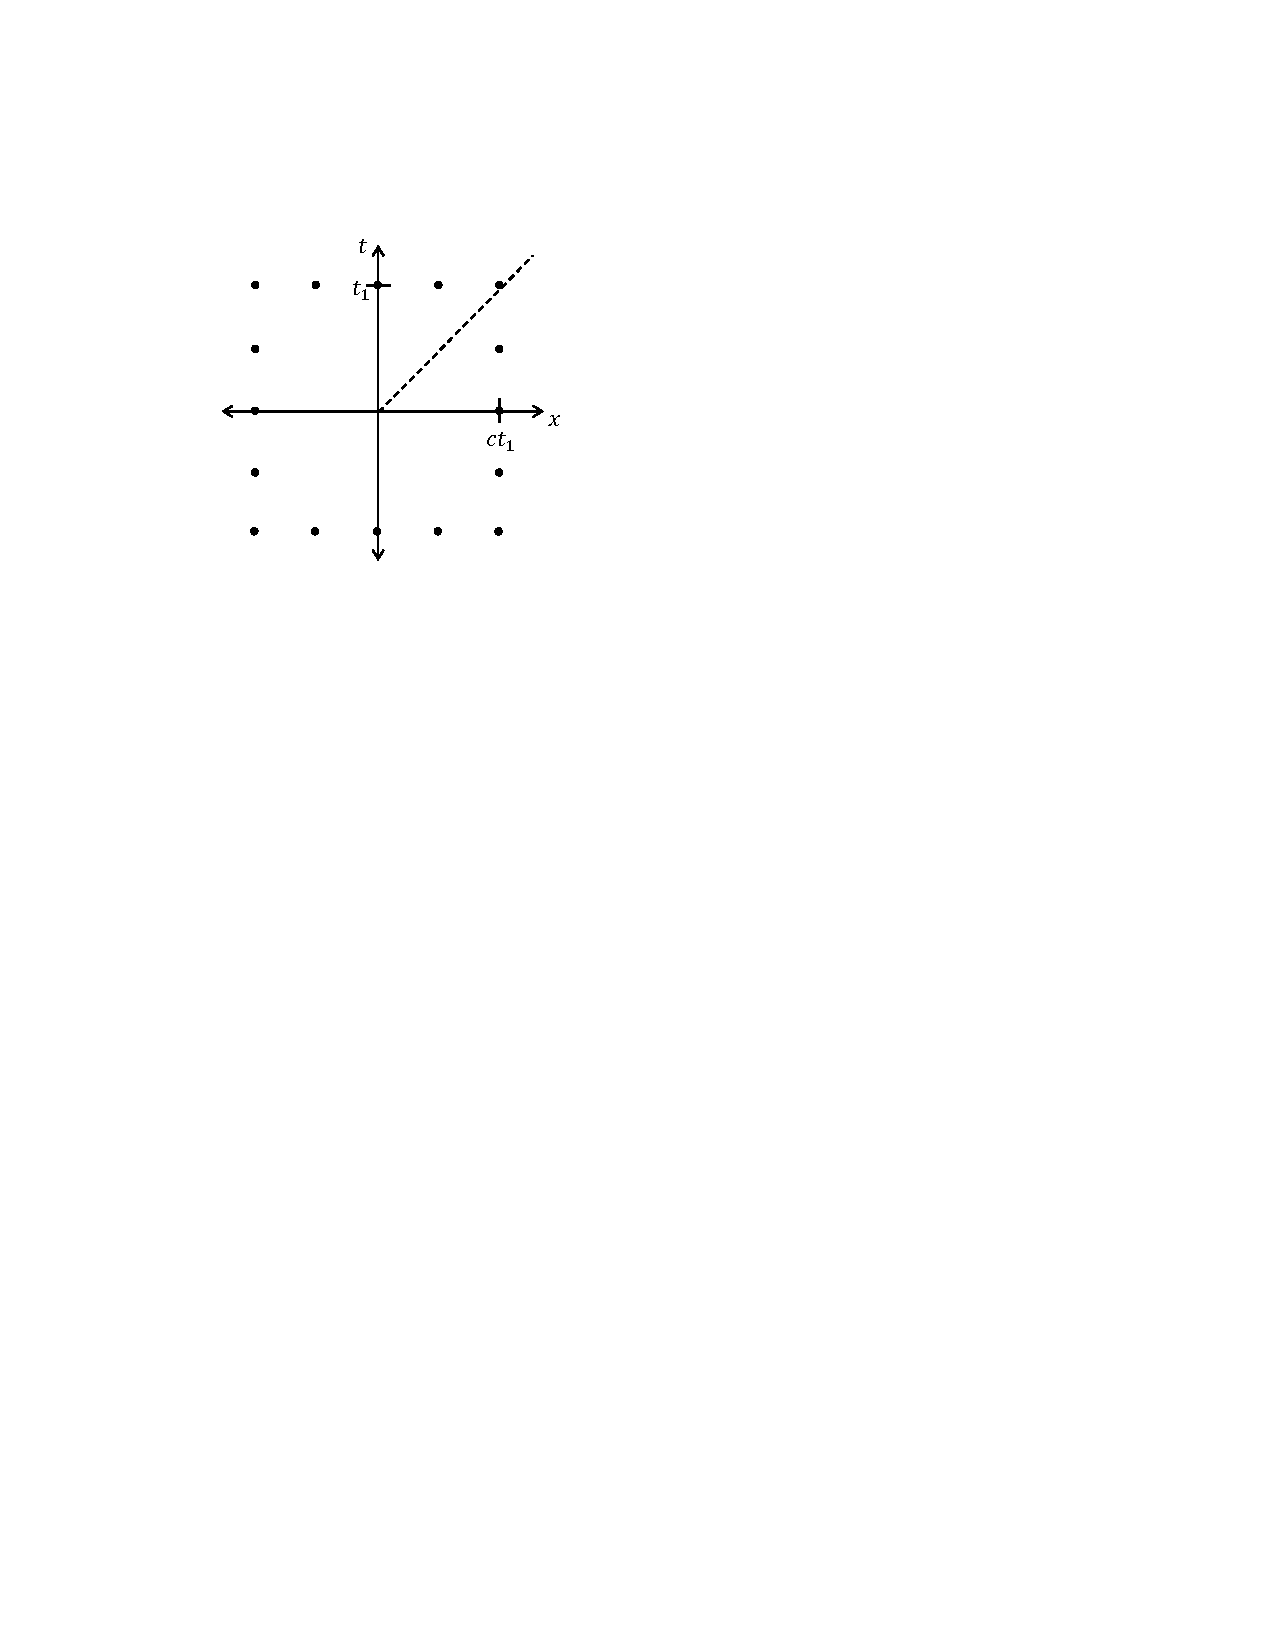
\includegraphics[scale=0.8]{M_problems/galilean_relativity/16_points.pdf}
\end{minipage}


\begin{Exercise}
\label{federation_and_romulans_prob}
A Federation spacecraft has had engine trouble and is drifting helplessly in space.  A Romulan spacecraft whizzes by at a constant velocity of $v=+0.2c$.  The Federation spacecraft radios the Romulan spacecraft and asks for help.  The Romulans answer back, ``We can't help you.  We are having engine trouble, and we are drifting helplessly in space.  We just saw you whiz by at $v=-0.2c$.  We were just about to radio you and ask for help.''  Are the reference frames of the two spacecraft equally valid?  Is there any way to tell only from the velocities of the two ships whether the Romulans are telling the truth?  Explain.
\end{Exercise}


\begin{Exercise}
The lettered parts of this problem are all related, in that they get at how the velocities of some different kinds of waves are seen in different reference frames.  \textbf{Draw a stick-figure cartoon for each situation below, along with labeled arrows showing the velocities given.} And, of course, answer the questions.
\begin{enumerate}[nosep,label=(\alph*)]
\item A luxurious limousine \href{https://veryfamousmagazine.com/glamorous-history-hot-tub-limo/}{includes an actual hot tub.}  
While the limousine is parked, you notice that when you splash your hand in the water, waves on the surface of the water travel from the back to the front at 2~m/s.  Suppose you splash your hand in the same way while the limousine is driving forward at 10~m/s.  In the reference frame of a person standing on the sidewalk as you pass by, what is the velocity of these water waves?
\item Now consider a different, regular-old-smelly-old limousine which does not include a hot tub, but is still rather long.  Inside the enclosed passenger area, sound travels at 343~m/s in air, just as it does outside.  Suppose you yell from the back of the limousine towards the driver in the front while the limousine is driving forward at 10~m/s.  In the reference frame of a person standing on the sidewalk as you pass by, what is the velocity of these sound waves?
\item Forget the limousine.  You are standing on a sidewalk, and you see your friend down the street from you, and you yell to her.  The wind is blowing from you towards your friend at 10~m/s.  In the reference frame of your friend, what is the velocity of the sound waves traveling towards her?
\item While you are still yelling to her, your friend starts to run towards you at a speedy 5~m/s.  Now, in the reference frame of your friend, what is the velocity of the sound waves traveling towards her?
\item Finally, suppose that you run towards your friend as well, at 3~m/s.  (And, to review, your friend is also running towards you at 5~m/s, and the wind is blowing towards your friend at 10~m/s.)  Now, in the reference frame of your friend, what is the velocity of the sound waves traveling towards her?
\end{enumerate}
\end{Exercise}
\begin{Answer}
(a) 12 m/s (b) 353 m/s (c) 353 m/s (d) 358 m/s (e) 358 m/s
\end{Answer}


\bigskip\bigskip\bigskip
\pagebreak[3]
\textbf{Answers to Selected {\thesubsection} Problems:}
\label{galilean_relativity_prob_answers}
%\shipoutExercise
\shipoutAnswer

\cleardoublepage